\documentclass[12pt,a4paper]{article}
\usepackage[utf8]{inputenc}
\usepackage{amsfonts}
\usepackage{amssymb}
\usepackage{graphicx}
\usepackage{float}

% sets margin
\usepackage[hmargin=3cm,vmargin=2.5cm]{geometry}

% creates landscape pages
\usepackage{pdflscape}
\usepackage{pdfpages}

%\renewcommand{\rmdefault}{phv} % Arial
\renewcommand{\sfdefault}{phv} % Arial

% defining settings for textpos
\usepackage[absolute]{textpos}
\setlength{\TPHorizModule}{\paperwidth}
\setlength{\TPVertModule}{\paperheight}

% headers / footers
\usepackage{fancyhdr}
\pagestyle{fancy}
\fancyhf{}
\rhead{Assignment 2A}
\lhead{CSG1207: Systems \& Database Design}
\rfoot{\thepage}
\lfoot{Martin Ponce, ID: 10371381}
\renewcommand{\footrulewidth}{0.5pt}

% defining landscape headers / footers
\fancypagestyle{fancylscape}{
	\fancyhf{}
	\renewcommand{\footrulewidth}{0pt}
	\renewcommand{\headrulewidth}{0pt}
	% header
	\begin{textblock}{0.05}[-0.5,-2](0,0)
		{\rotatebox{90}{CSG1207: Systems \& Database Design}}
	\end{textblock}
		\begin{textblock}{0.05}[-0.5,-1](0,0)
		{\rotatebox{90}{Assignment 2A}}
	\end{textblock}
	\begin{textblock}{0.05}[-1,-0.109](0,0)
		{\rotatebox{90}{\rule{24.2cm}{0.5pt}}}
	\end{textblock}
	% footer
	\begin{textblock}{0.05}[-19,-4.28](0,0)
		{\rotatebox{90}{Martin Ponce, ID: 10371381}}
	\end{textblock}
		\begin{textblock}{0.05}[-19,-12.8](0,0)
		{\rotatebox{90}{\thepage}}
	\end{textblock}
		\begin{textblock}{0.05}[-18.7,-0.109](0,0)
		{\rotatebox{90}{\rule{24.2cm}{0.5pt}}}
	\end{textblock}
}

% adjusts padding between caption and figure
\setlength{\belowcaptionskip}{10pt}

% adds links to references and colors them blue
\usepackage{hyperref}
\hypersetup{colorlinks=true,
			linkcolor=blue,
			citecolor=black,
			urlcolor=blue}

% apa style referencing
\usepackage[sectionbib, natbibapa]{apacite}
\usepackage{chbibref}

% underlining text
\usepackage[normalem]{ulem}

% \citetapos for possesive citations
\newcommand{\citetapos}[1]{\citeauthor{#1}{\textcolor{black}{'s}} \citeyearpar{#1}}

% add multiline comments \begin{comment} \end{comment}
\usepackage{verbatim}

% front matter
\title{Edith Cowan University\\CSG1207\\Systems \& Database Design\\Assignment 2A}
\author{Martin Ponce\\Student 10371381\\\\Tutor: Greg Baatard}
\date{\today}

\begin{document}

% title page
\newpage
\null  % Empty line
\nointerlineskip  % No skip for prev line
\vfill
\let\snewpage \newpage
\let\newpage \relax
\maketitle
\thispagestyle{empty}
\let \newpage \snewpage
\vfill

% toc
\newpage
\tableofcontents
\thispagestyle{fancy}

\newpage
\section{Pizza store database design brief}

You are required to design and create a database for a pizza store. The database must encompass the customers, staff, pizza details, and the pizza orders made by customers. You have the following information about the way the store operates:

\begin{itemize}
\item Customer details must be recorded. This includes a customer ID number, name, address and email. Customer details are recorded when they make their first order.
\item Staff details must be recorded. This includes a staff ID number, first name, last name, date of birth and phone number.
	\begin{itemize}
	\item Each staff member may have a supervisor, which is another staff member. A staff member may supervise many other staff members. Not all staff have a supervisor.
	\end{itemize}
\item The details of pizza orders must be recorded. This includes an order ID number, the date and time that the order was placed, the ID number of the customer who made the order, and the ID number of the staff member who took the order.
	\begin{itemize}
	\item The table also needs to contain the staff ID number of the staff who delivered the order. Since the pizza order will be recorded before the pizzas are delivered, this value will originally be empty.
	\item Each order can contain multiple pizzas.
	\end{itemize}
\item The store has divided their pizza selection into ``ranges'' (e.g. ``traditional'' and ``gourmet'') to simplify pricing. All of the pizzas in a range have the same price.
	\begin{itemize}
	\item The database must store an ID, name and price for each range.
	\end{itemize}
\item The details of the types of pizza available must be recorded. This includes a pizza ID number, the pizza’s name, a description and a foreign key identifying which pizza range it is in.
\item The database also needs two tables to store the details of crust types and sauce types that can be chosen when ordering a pizza. Some crust/sauce types attract a surcharge.
	\begin{itemize}
	\item These tables require an ID number, name and surcharge (default of 0) column.
	\item When ordering a pizza, a customer must choose which crust and sauce they want.
	\end{itemize}
\item The database must track which pizzas were ordered in which orders. This will involve:
	\begin{itemize}
	\item An auto-incrementing ordered pizza ID number.
	\item A foreign key identifying the order that this pizza is part of.
	\item A foreign key identifying which pizza was chosen.
	\item A foreign key identifying which crust was chosen.
	\item A foreign key identifying which sauce was chosen.
	\item A ``ready'' column containing a ``Y'' or ``N'' to indicate whether the pizza has been made and cooked yet (default of ``N'').
	\end{itemize}
\end{itemize}

\section{Assumptions}

\subsection{ER diagrams}

\begin{itemize}
\item A Customer must make at least one CustomerOrder to exist on database
\item A CustomerOrder must contain at least one PizzaOrder
\item A PizzaOrder must include one PizzaType selection
	\begin{itemize}
	\item It is possible that a PizzaType may never be selected for a PizzaOrder
	\end{itemize}
\item A PizzaOrder must include one PizzaCrust selection
	\begin{itemize}
	\item It is possible that a PizzaCrust may never be selected for a PizzaOrder
	\end{itemize}
\item A PizzaOrder must include one PizzaSauce selection
	\begin{itemize}
	\item It is possible that a PizzaSauce may never be selected for a PizzaOrder
	\end{itemize}
\item A PizzaType must include one PizzaRange selection
	\begin{itemize}
	\item It is possible that a PizzaRange may never be selected for a PizzaOrder
	\end{itemize}
\item A staff member may be a supervisor to many staff members
	\begin{itemize}
	\item A staff member may only have one supervisor
	\item Some staff may not have a supervisor
	\end{itemize}
\item A staff member may not deliver any pizzas
\end{itemize}

\subsection{Data dictionary}

\begin{itemize}
\item Database will not be implented in SQL 2005
\item Total number of Staff will not exceed 255
\item Total number of Customers will not exceed 32,767
\item Price of PizzaCrust or PizzaSauce will each not exceed \$9.99
\item Price of PizzaRange will not exceed \$99.99
\item Total number of PizzaCrust, PizzaSauce or PizzaRange will each not exceed 255
\item Total number of CustomerOrder or PizzaOrder will each not exceed 2,147,483,647
\end{itemize}
\newpage
\section{Logical E-R diagram}

Updated table/column names per implementation.

\begin{figure}[H]
\centering
\caption{Pizza Store Logical E-R Diagram}
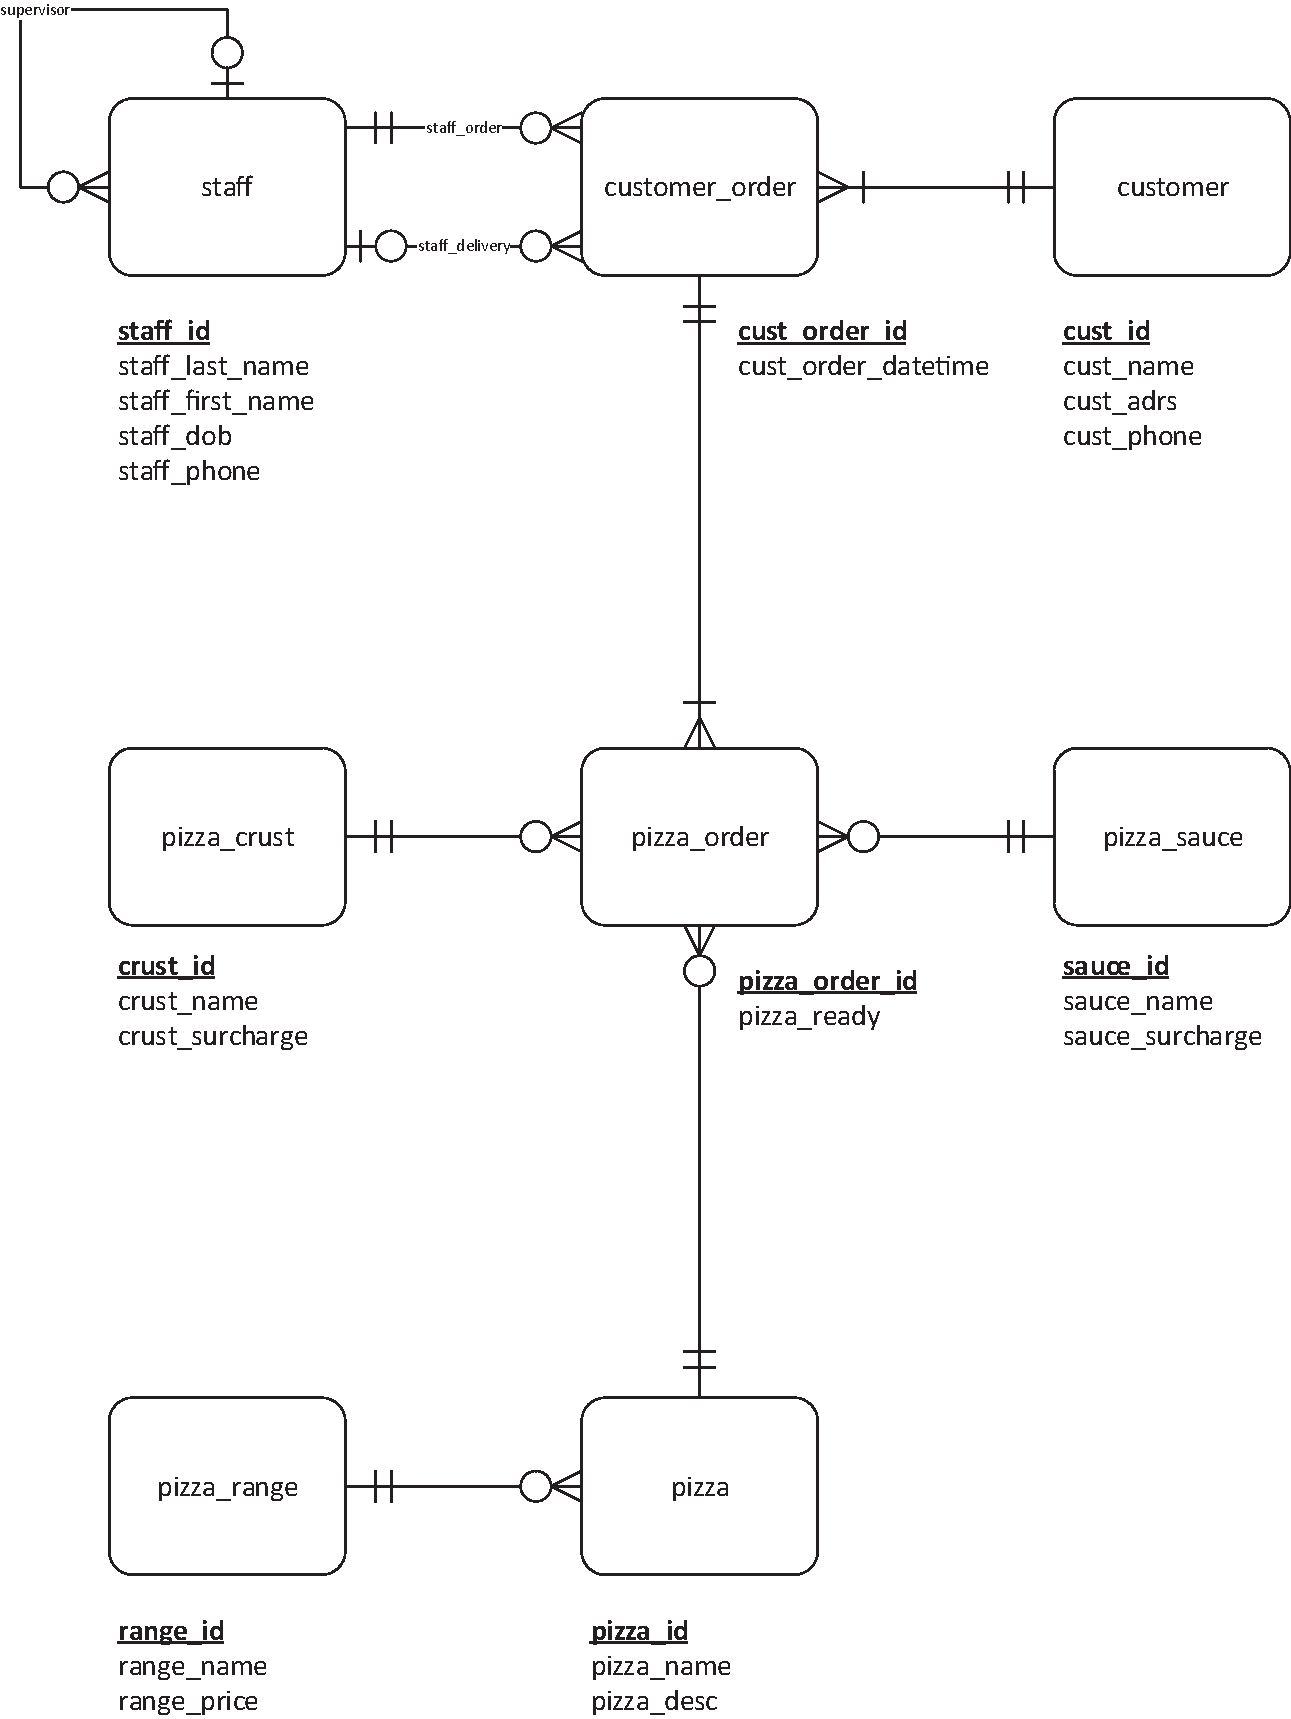
\includegraphics[scale=0.6]{./img/CSG1207_A1_PONCE_TASK_4_ADVLER_PIZZA.pdf}
\end{figure}
\newpage
\section{Physical E-R diagram}

Updated table/column names per implementation.

\begin{figure}[H]
\centering
\caption{Pizza Store Physical E-R Diagram}
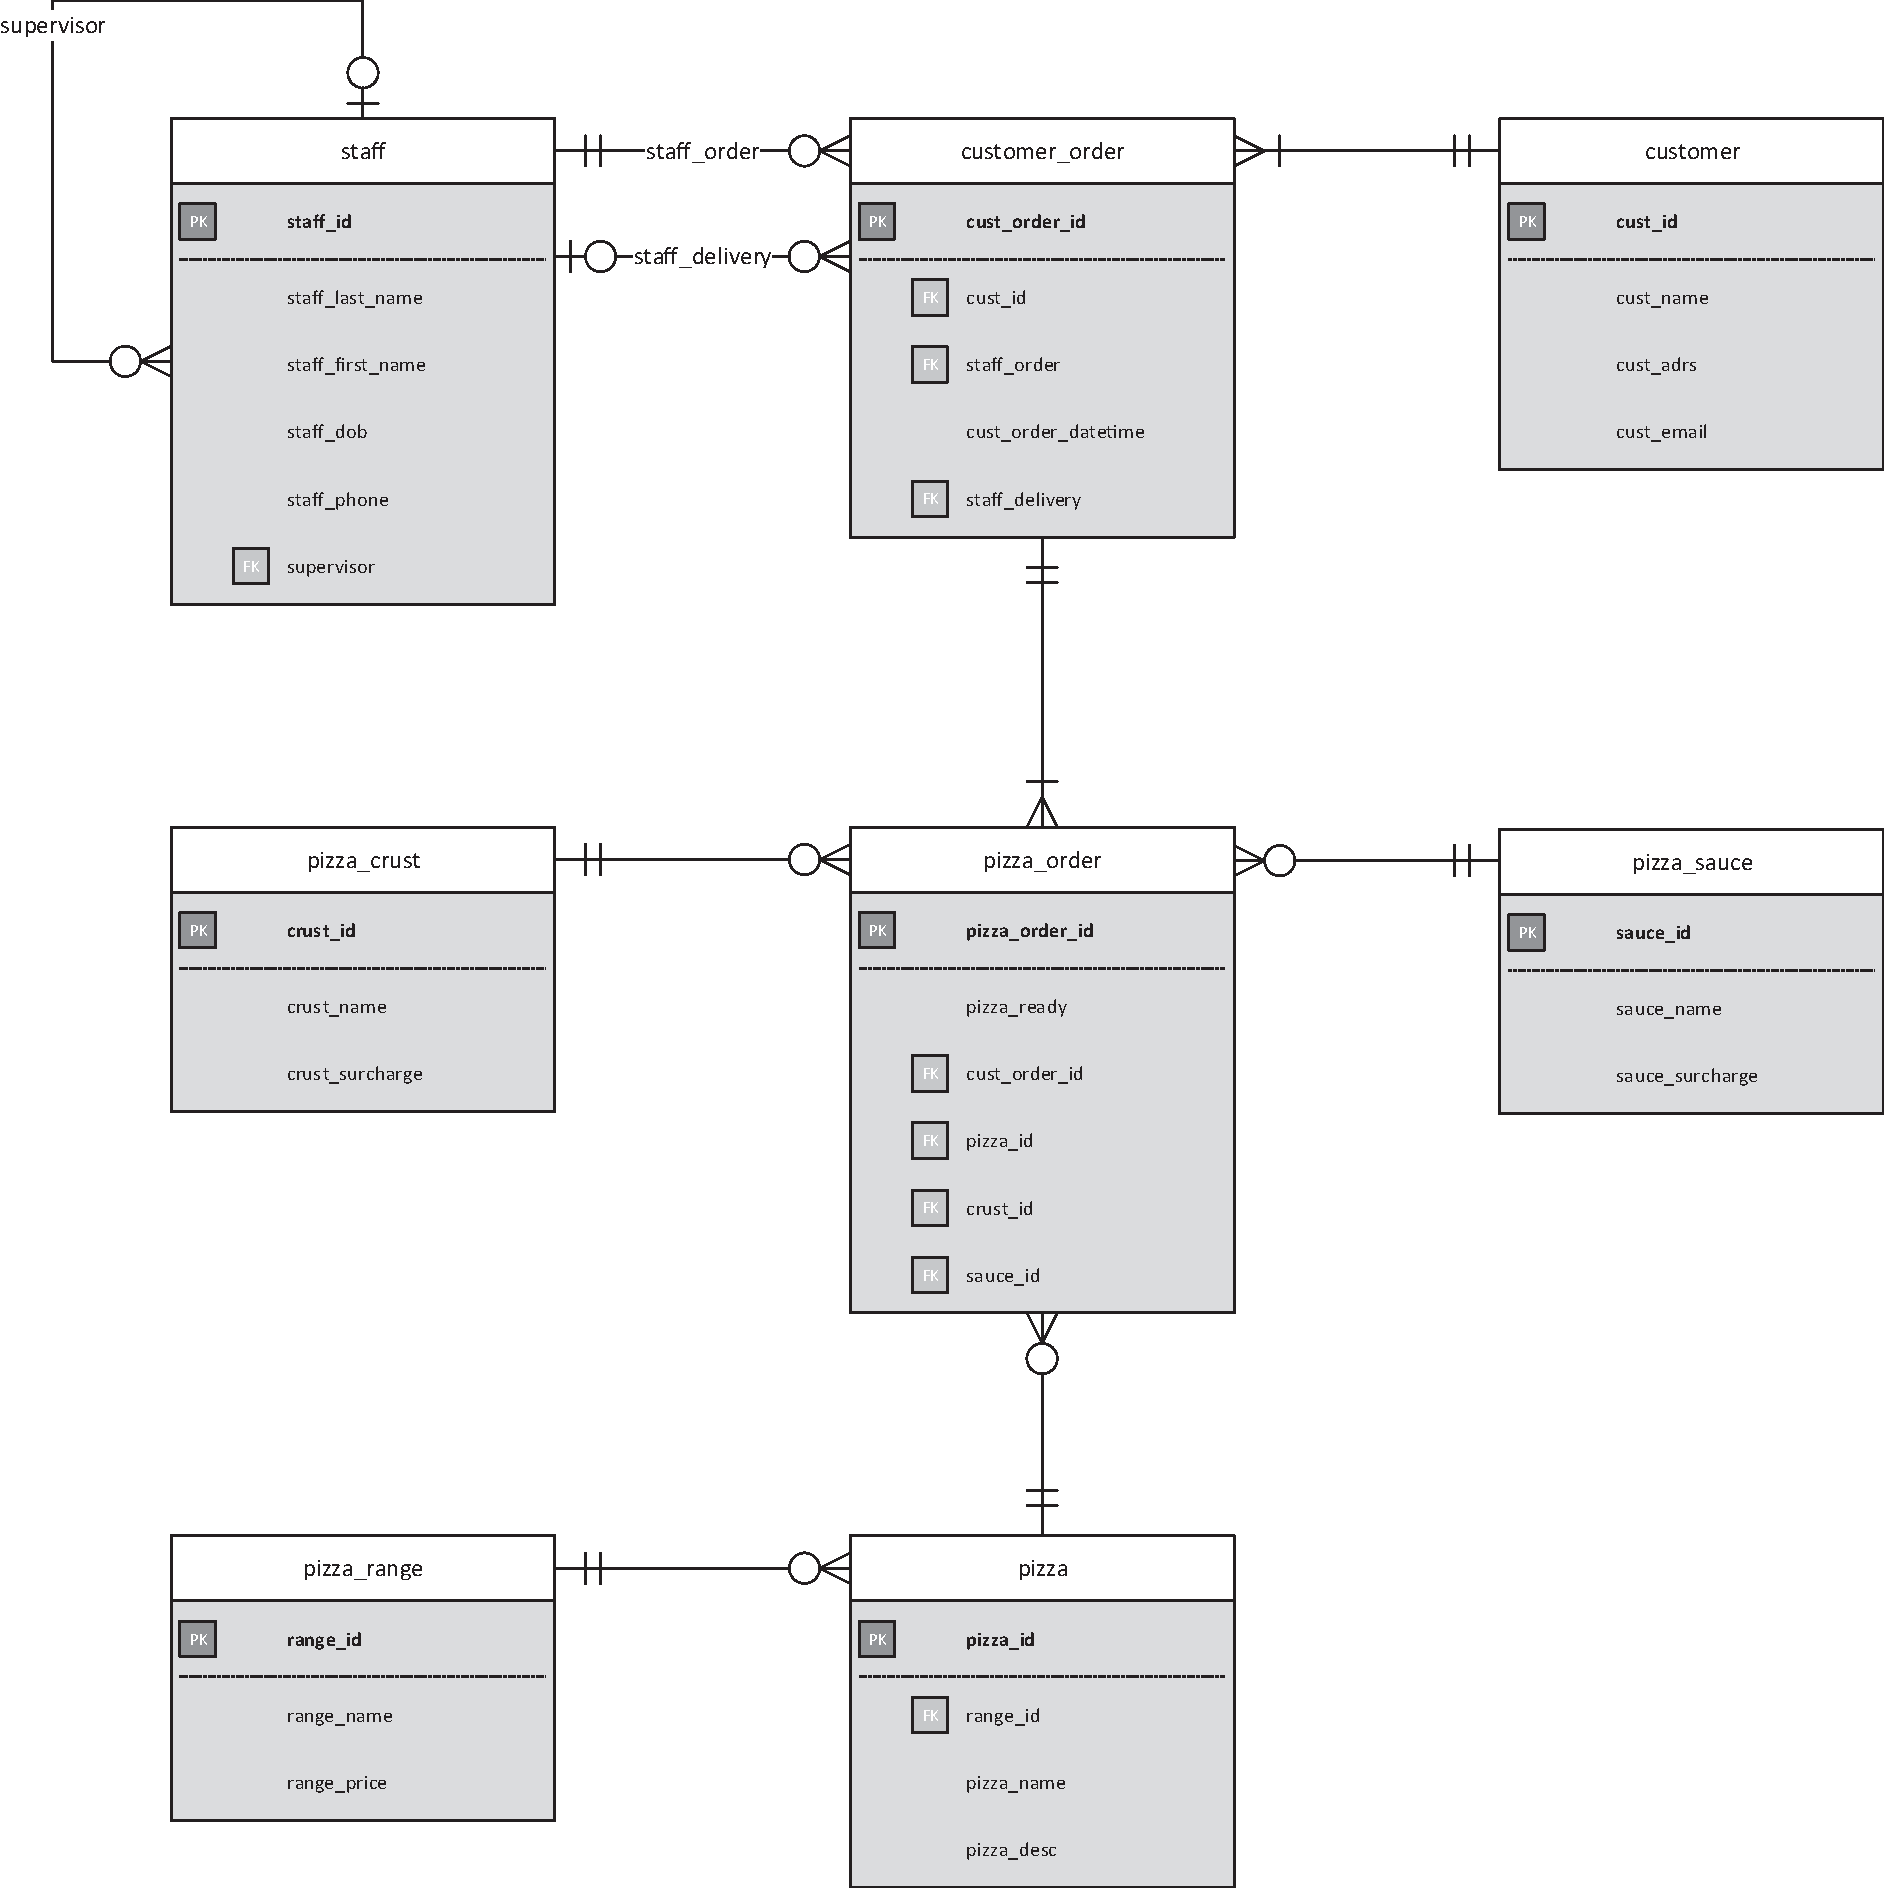
\includegraphics[scale=0.45]{./img/CSG1207_A1_PONCE_TASK_4_ADVPER_PIZZA.pdf}
\end{figure}
\newpage
\section{Data dictionary \& creation order}


\begin{table}[H]
  \centering
  \caption{\textbf{``staff''} stores details about staff}
  	\begin{footnotesize}
    \begin{tabular}{lllll}
    \textbf{Column name} & \textbf{Type/Length} & \textbf{Null} & \textbf{Constraints} & \textbf{Other} \\
    staff\_id & TINYINT   & NOT NULL & PK    & IDENTITY \\
    staff\_last\_name & VARCHAR(20) & NOT NULL &       &  \\
    staff\_first\_name & VARCHAR(20) & NOT NULL &       &  \\
    staff\_dob & DATE  & NOT NULL &       &  \\
    staff\_phone & VARCHAR(20) & NOT NULL &       &  \\
    supervisor & TINYINT   & NULL & FK (staff.staff\_id) &  \\
    %\bottomrule
    \end{tabular}%
    \end{footnotesize}
  \label{tab:addlabel}%
\end{table}%

\begin{table}[H]
  \centering
  \caption{\textbf{``customer''} stores details about customer}
  	\begin{footnotesize}
    \begin{tabular}{lllll}
    \textbf{Column name} & \textbf{Type/Length} & \textbf{Null} & \textbf{Constraints} & \textbf{Other} \\
    cust\_id & SMALLINT   & NOT NULL & PK    & IDENTITY \\
    cust\_name & VARCHAR(50) & NOT NULL &       &  \\
    cust\_adrs & TEXT  & NOT NULL &       &  \\
    cust\_phone & VARCHAR(20) & NOT NULL &       &  \\
    \end{tabular}%
    \end{footnotesize}
  \label{tab:addlabel}%
\end{table}%

\begin{table}[H]
  \centering
  \caption{\textbf{``customer\_order''} stores details about customer order}
  	\begin{footnotesize}
    \begin{tabular}{lllll}
    \textbf{Column name} & \textbf{Type/Length} & \textbf{Null} & \textbf{Constraints} & \textbf{Other} \\
    cust\_order\_id & INT   & NOT NULL & PK    & IDENTITY \\
    cust\_id & SMALLINT   & NOT NULL & FK (customer.cust\_id) &  \\
    staff\_order & TINYINT   & NOT NULL & FK (staff.staff\_id) &  \\
    cust\_order\_datetime & DATETIME & NOT NULL &       &  \\
    staff\_delivery & TINYINT   & NULL  & FK (staff.staff\_id) &  \\
    \end{tabular}%
    \end{footnotesize}
  \label{tab:addlabel}%
\end{table}%

\begin{table}[H]
  \centering
  \caption{\textbf{``pizza\_crust''} stores details about pizza crust}
  	\begin{footnotesize}
    \begin{tabular}{lllll}
    \textbf{Column name} & \textbf{Type/Length} & \textbf{Null} & \textbf{Constraints} & \textbf{Other} \\
    pizza\_crust\_id & TINYINT   & NOT NULL & PK    & IDENTITY \\
    pizza\_crust\_name & VARCHAR(20) & NOT NULL &       &  \\
    surcharge & SMALLMONEY & NOT NULL &       &  \\
    \end{tabular}%
    \end{footnotesize}
  \label{tab:addlabel}%
\end{table}%

\begin{table}[H]
  \centering
  \caption{\textbf{``pizza\_sauce''} stores details about pizza sauce}
  	\begin{footnotesize}
    \begin{tabular}{lllll}
    \textbf{Column name} & \textbf{Type/Length} & \textbf{Null} & \textbf{Constraints} & \textbf{Other} \\
    pizza\_sauce\_id & TINYINT   & NOT NULL & PK    & IDENTITY \\
    pizza\_sauce\_name & VARCHAR(20) & NOT NULL &       &  \\
    surcharge & SMALLMONEY & NOT NULL &       &  \\
    \end{tabular}%
    \end{footnotesize}
  \label{tab:addlabel}%
\end{table}%

\begin{table}[H]
  \centering
  \caption{\textbf{``pizza\_range''} stores details about pizza range}
  	\begin{footnotesize}
    \begin{tabular}{lllll}
    \textbf{Column name} & \textbf{Type/Length} & \textbf{Null} & \textbf{Constraints} & \textbf{Other} \\
    pizza\_range\_id & TINYINT   & NOT NULL & PK    & IDENTITY \\
    pizza\_range\_name & VARCHAR(20) & NOT NULL &       &  \\
    pizza\_range\_price & SMALLMONEY & NOT NULL &       &  \\
    \end{tabular}%
    \end{footnotesize}
  \label{tab:addlabel}%
\end{table}%

\begin{table}[H]
  \centering
  \caption{\textbf{``pizza\_type''} stores details about pizza type}
  	\begin{footnotesize}
    \begin{tabular}{lllll}
    \textbf{Column name} & \textbf{Type/Length} & \textbf{Null} & \textbf{Constraints} & \textbf{Other} \\
    pizza\_type\_id & TINYINT   & NOT NULL & PK    & IDENTITY \\
    pizza\_range\_id & TINYINT   & NOT NULL & FK (pizza\_range.pizza\_range\_id) &  \\
    pizza\_name & VARCHAR(20) & NOT NULL &       &  \\
    pizza\_desc & TEXT  & NOT NULL &       &  \\
    \end{tabular}%
    \end{footnotesize}
  \label{tab:addlabel}%
\end{table}%

\begin{table}[H]
  \centering
  \caption{\textbf{``pizza\_order''} stores details about pizza order}
  	\begin{footnotesize}
    \begin{tabular}{lllll}
    \textbf{Column name} & \textbf{Type/Length} & \textbf{Null} & \textbf{Constraints} & \textbf{Other} \\
    pizza\_order\_id & INT   & NOT NULL & PK    & IDENTITY \\
    pizza\_ready & CHAR(1)   & NOT NULL & CHECK (pizza\_ready IN (`Y', `N')) & DEFAULT `N' \\
    cust\_order\_id & INT   & NOT NULL & FK (customer.cust\_id) &  \\
    pizza\_type\_id & TINYINT   & NOT NULL & FK (pizza\_type.pizza\_type\_id) &  \\
    pizza\_crust\_id & TINYINT   & NOT NULL & FK (pizza\_crust.pizza\_crust\_id) &  \\
    pizza\_sauce\_id & TINYINT   & NOT NULL & FK (pizza\_sauce.pizza\_sauce\_id) &  \\
    \end{tabular}%
    \end{footnotesize}
  \label{tab:addlabel}%
\end{table}%

\newpage
\urlstyle{rm}
%\setbibref{\textsf{References}}
\bibliographystyle{apacite}
\addcontentsline{toc}{section}{References}
%\bibliography{./bib/Year 1-Sem 2-CSI1101-A1}

\end{document}